

\section{Experiments and Results}	
In the following we will present three experiments from the paper that we tried to reproduce and tried to mimic as closely as possible. 
All the experiments use a two-layered or three-layered structure which include either a NPTN layer, a Convolutional layer or a RotNet layer in each layer. The structure for the two-layered network is shown in Figure \ref{pic:net_structure}. The last softmax layer is not described in the paper, but was added by us [WHY softmax, because it's standard]. 

\begin{figure}
	\begin{center}
	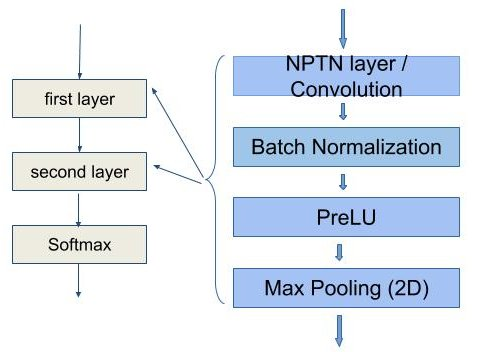
\includegraphics[scale=0.35]{result_images/network_structure.jpg}
	\caption{Structure of a two layered network.}
	\label{pic:network_structure}
	\end{center}
\end{figure}

\subsection{Experiments on CIFAR10}
The first experiment used the CIFAR10 dataset [CITE]. A CNN and several NPTNs with different values for G are tested. The dimension of the NPTNs is changed for the different values of G such that all networks have the same amount of filters.
The paper describes in detail the setup of the experiments regarding learning rate, data preprocessing and network dimensions. However other important information as filter size and loss function is missing. 
For the filtersize we used 5, since in the other experiments, the paper mentions  filtersizes of 3,5 or 7 and 5 often shows the best performance for the NPTNs. 
In Figure \ref{pic:first_experiment} we show the results from the paper next to our experimental results. For the loss function we chose Negative Log Likelihood Loss (NLLL) [WHY]. 
However we did not get any comparable loss values as in the paper. Comparing the loss values of the networks to each other, in the paper, all NPTNs perform better than the CNN. In our results, only one of the NPTNs performs better.
Since we are not sure if the loss used in the paper is the same, we also calculated the accuracy of the networks. The values are consistent with the loss for this experiment, so for each network if the loss is lower, then the accuracy is higher compared to other networks.

\begin{figure}
	\begin{center}
	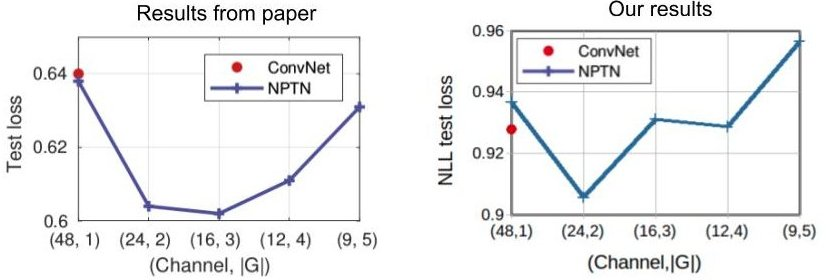
\includegraphics[scale=0.35]{result_images/experiment1.jpg}
	\caption{The first experiment}
	\label{pic:first_experiment}
	\end{center}
\end{figure}

TRAIN vs TEST ERROR?

\section{Rotation Experiments on MNIST}
The second experiment from the paper compares a CNN and several NPTNs. Again the dimensions are chosen in a way that matches the values in the paper and leads to the same amount of filters for all networks. 
This experiment uses the MNIST dataset [CITE] where all images from training and test set were randomly rotated up to a certain degree. 
The paper shows the results from various maximal rotation degrees. we picked the two strongest rotations, since the performance difference between NPTNs and CNNs was the biggest there and performed our own experiments, adding also RotNets for comparison.
The Paper did specify the data preprocessing in detail, but didn't give new instructions for learning rate, so we kept the same experiment setup as in the first experiment.
The results from our experiments are shown in Figure \ref{pic:second_experiment}. [TODO: new graphic?]


\section{Three-layered-networks}
This experiment from the paper compares three-layered NPTNs and CNNs of the CIFAR10 dataset [CITE]. 
The network dimensions are not described well and the paper states that the amount of parameters for those networks is similar, but not exactly the same as in the previous experiments. 
Therefore we determined possible dimensions for the amount of channels in the NPTNs and CNNs. 
Again no new learning rate was given for this experiment, so we initially tried with the same experimental setup as in the first two experiments, but using this and the dimensions that seemed likely from the paper led the networks to overfit greatly and the loss values did not improve. 
Therefore we reduced the amount of parameters and the learning rate and achieved a result, which had less generalization error. 
Different than in the first two experiments accuracy and loss are not consistent anymore. While the loss starts getting worse after some iteration, the accuracy stays approximately stable and we therefore used the accuracy to compare the networks.
[TODO show results]

\section{Experiments for RotNet}
The final experiment was designed by us to see if RotNet was able to perform one of the ideas behind its design: the ability to be invariant to rotations without learning them. For this we copied the setup of the MNIST rotation experiment with the difference, that this time we only rotated the test set. The results are shown in Figure [FIG]. 
